\documentclass[8pt,aspectratio=169]{beamer}
\usepackage[utf8]{inputenc}
\usepackage{graphicx}
\usepackage{amsmath,amssymb}
\usepackage{algorithm2e}
\usepackage{listings}
\usepackage{xcolor}
\usepackage{tikz}
\usepackage{pgfplots}
\pgfplotsset{compat=1.17}
\usepackage{subfigure}
\usepackage{hyperref}
\usepackage{tcolorbox}
\usepackage{fontawesome5}

% Theme settings
\usetheme{Frankfurt}
\usecolortheme{seahorse}
\setbeamertemplate{navigation symbols}{}
\setbeamertemplate{footline}[frame number]
\setbeamertemplate{section in toc}[sections numbered]
\setbeamertemplate{subsection in toc}[subsections numbered]

% Custom colors
\definecolor{darkblue}{RGB}{0,51,102}
\definecolor{lightblue}{RGB}{173,216,230}
\definecolor{codegreen}{RGB}{0,128,0}
\definecolor{codegray}{RGB}{150,150,150}
\definecolor{codepurple}{RGB}{128,0,128}
\definecolor{backcolor}{RGB}{245,245,245}
\definecolor{prereqblue}{RGB}{230,240,255}
\definecolor{misconred}{RGB}{255,230,230}
\definecolor{checkgreen}{RGB}{230,255,230}

% Code listing settings
\lstset{
    backgroundcolor=\color{backcolor},
    basicstyle=\ttfamily\tiny,
    breakatwhitespace=false,
    breaklines=true,
    captionpos=b,
    commentstyle=\color{codegreen},
    keywordstyle=\color{blue},
    numberstyle=\tiny\color{codegray},
    stringstyle=\color{codepurple},
    showstringspaces=false,
    frame=single,
    numbers=left,
    language=Python
}

% Custom commands for BSc level
\newcommand{\highlight}[1]{\textcolor{blue}{\textbf{#1}}}
\newcommand{\eqbox}[1]{\begin{tcolorbox}[colback=blue!5!white,colframe=blue!75!black]#1\end{tcolorbox}}
\newcommand{\prereq}[1]{\begin{tcolorbox}[colback=prereqblue,colframe=blue!50!black,title={\faIcon{book} Prerequisite}]#1\end{tcolorbox}}
\newcommand{\misconception}[1]{\begin{tcolorbox}[colback=misconred,colframe=red!50!black,title={\faIcon{exclamation-triangle} Common Misconception}]#1\end{tcolorbox}}
\newcommand{\checkpoint}[1]{\begin{tcolorbox}[colback=checkgreen,colframe=green!50!black,title={\faIcon{check-circle} Check Your Understanding}]#1\end{tcolorbox}}
\newcommand{\motivation}[1]{\begin{tcolorbox}[colback=yellow!10!white,colframe=orange!75!black,title={\faIcon{lightbulb} Why This Matters}]#1\end{tcolorbox}}
\newcommand{\given}{\mid}
\newcommand{\prob}[1]{P(#1)}
\DeclareMathOperator*{\argmax}{arg\,max}
\DeclareMathOperator*{\softmax}{softmax}

\title[Week 4: Seq2Seq]{Natural Language Processing}
\subtitle{Week 4: Sequence-to-Sequence Models}
\institute{Breaking the Fixed-Length Barrier}
\author{}
\date{}

\begin{document}

% Title slide
\begin{frame}
    \titlepage
\end{frame}

% Learning Objectives
\begin{frame}{Learning Objectives}
    \begin{columns}[T]
        \begin{column}{0.5\textwidth}
            \textbf{By the end of this lecture, you will:}
            \begin{enumerate}
                \item Understand why translation is hard for neural networks
                \item Design encoder-decoder architectures
                \item Identify the information bottleneck problem
                \item Master the attention mechanism
                \item Implement your own seq2seq model
            \end{enumerate}
        \end{column}
        \begin{column}{0.5\textwidth}
            \prereq{
                \textbf{Required Knowledge:}
                \begin{itemize}
                    \item RNNs and LSTMs (Week 3)
                    \item Backpropagation basics
                    \item Softmax function
                    \item Python/NumPy
                \end{itemize}
            }
        \end{column}
    \end{columns}
\end{frame}

% Table of Contents
\begin{frame}{Week 4 Overview}
    \tableofcontents
\end{frame}

%=====================================
% PART 1: THE VARIABLE-LENGTH CHALLENGE
%=====================================

\section{Part 1: The Variable-Length Challenge}

\begin{frame}[t]{Why Can't We Just Use RNNs?}
    \motivation{
        You learned RNNs last week. Why can't we use them for translation?
    }
    
    \vspace{0.5em}
    \textbf{The Fundamental Problem:}
    
    \begin{columns}[T]
        \begin{column}{0.5\textwidth}
            \textbf{What RNNs expect:}
            \begin{itemize}
                \item Input: Sequence of length $n$
                \item Output: Sequence of length $n$
                \item One output per input!
            \end{itemize}
            
            \vspace{0.5em}
            \textbf{Example that works:}
            \begin{itemize}
                \item POS tagging: word $\rightarrow$ tag
                \item "The cat sat" $\rightarrow$ "DET NOUN VERB"
                \item 3 inputs $\rightarrow$ 3 outputs \checkmark
            \end{itemize}
        \end{column}
        \begin{column}{0.5\textwidth}
            \textbf{What translation needs:}
            \begin{itemize}
                \item Input: Sequence of length $n$
                \item Output: Sequence of length $m$
                \item $n \neq m$ in general!
            \end{itemize}
            
            \vspace{0.5em}
            \textbf{Example that fails:}
            \begin{itemize}
                \item Translation: English $\rightarrow$ French
                \item "I love you" $\rightarrow$ "Je t'aime"
                \item 3 inputs $\rightarrow$ 2 outputs \texttimes
            \end{itemize}
        \end{column}
    \end{columns}
    
    \vspace{0.5em}
    \checkpoint{
        Can you think of other tasks where input and output lengths differ?
    }
\end{frame}

\begin{frame}[t]{Real Translation Examples}
    \textbf{Let's see why word-by-word translation fails:}
    
    \begin{center}
    \begin{tabular}{|l|l|c|c|}
        \hline
        \textbf{English} & \textbf{Target Language} & \textbf{EN Words} & \textbf{Target Words} \\
        \hline
        I love you & Je t'aime (French) & 3 & 2 \\
        I love you & Ich liebe dich (German) & 3 & 3 \\
        I love you & Aishiteru (Japanese) & 3 & 1 \\
        I love you & Wo ai ni (Chinese) & 3 & 3 \\
        I love you & Te amo (Spanish) & 3 & 2 \\
        \hline
    \end{tabular}
    \end{center}
    
    \vspace{0.5em}
    \textbf{Even worse with longer sentences:}
    
    \begin{itemize}
        \item EN: "The International Conference on Machine Learning" (6 words)
        \item FR: "La Conférence Internationale sur l'Apprentissage Automatique" (6 words)
        \item DE: "Die Internationale Konferenz für Maschinelles Lernen" (6 words)
        \item But word alignment is completely different!
    \end{itemize}
    
    \misconception{
        \textbf{Wrong:} "We can just pad shorter sequences with zeros!"\\
        \textbf{Problem:} Where do you pad? Beginning? End? How many zeros?\\
        The model has no way to know the target length beforehand!
    }
\end{frame}

\begin{frame}[t]{Evolution of Translation Approaches}
    \begin{center}
    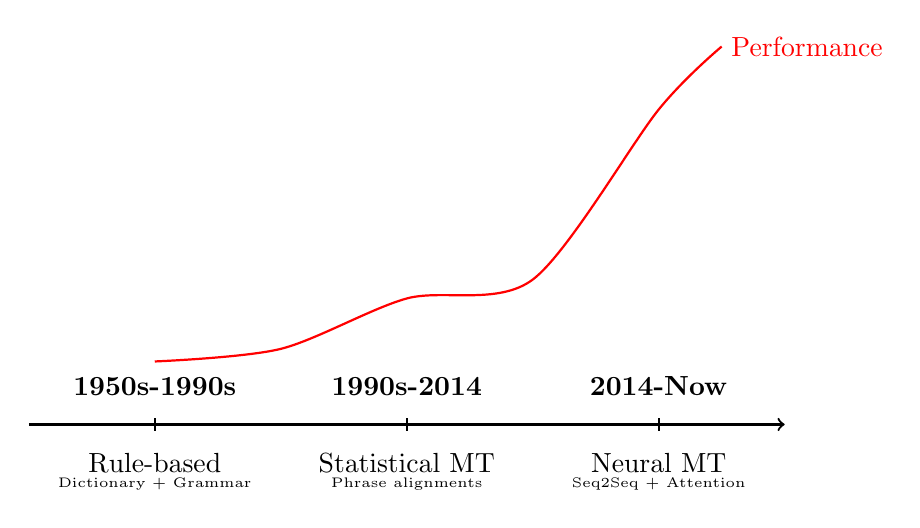
\begin{tikzpicture}[scale=0.8]
        % Timeline
        \draw[thick, ->] (0,0) -- (12,0);
        
        % Eras
        \node[above] at (2,0.3) {\textbf{1950s-1990s}};
        \node[below] at (2,-0.3) {Rule-based};
        \node[below] at (2,-0.7) {\tiny Dictionary + Grammar};
        
        \node[above] at (6,0.3) {\textbf{1990s-2014}};
        \node[below] at (6,-0.3) {Statistical MT};
        \node[below] at (6,-0.7) {\tiny Phrase alignments};
        
        \node[above] at (10,0.3) {\textbf{2014-Now}};
        \node[below] at (10,-0.3) {Neural MT};
        \node[below] at (10,-0.7) {\tiny Seq2Seq + Attention};
        
        % Markers
        \foreach \x in {2,6,10} {
            \draw[thick] (\x,-0.1) -- (\x,0.1);
        }
        
        % Performance curve
        \draw[thick, red] plot[smooth] coordinates {
            (2,1) (4,1.2) (6,2) (8,2.3) (10,5) (11,6)
        };
        \node[red, right] at (11,6) {Performance};
    \end{tikzpicture}
    \end{center}
    
    \vspace{0.5em}
    \textbf{The 2014 Breakthrough:}
    \begin{itemize}
        \item Sutskever, Vinyals, and Le: "Sequence to Sequence Learning with Neural Networks"
        \item Key insight: \highlight{Separate the reading from the writing!}
        \item Use two different networks: Encoder and Decoder
    \end{itemize}
    
    \motivation{
        This single idea revolutionized not just translation, but also chatbots, summarization, and code generation!
    }
\end{frame}

\begin{frame}[t]{The Brilliant Insight}
    \textbf{How humans translate:}
    \begin{enumerate}
        \item Read and \highlight{understand} the entire sentence
        \item Form a mental \highlight{representation} of the meaning
        \item \highlight{Generate} the translation from that understanding
    \end{enumerate}
    
    \vspace{0.5em}
    \textbf{The Seq2Seq approach (mimics humans):}
    
    \begin{center}
    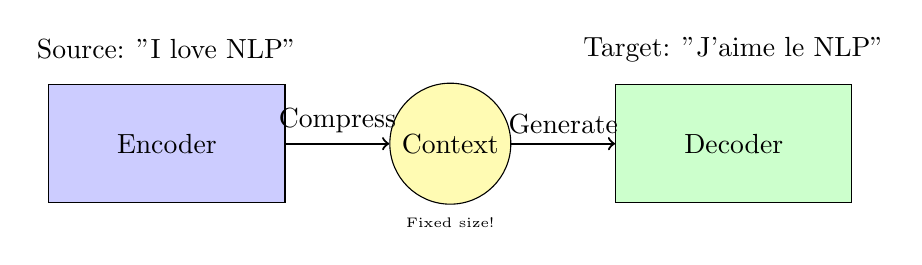
\begin{tikzpicture}[scale=0.9]
        % Encoder
        \node[draw, rectangle, minimum width=3cm, minimum height=1.5cm, fill=blue!20] (encoder) at (0,0) {Encoder};
        \node[above of=encoder, node distance=1.2cm] {Source: "I love NLP"};
        
        % Context vector
        \node[draw, circle, fill=yellow!30] (context) at (4,0) {Context};
        \node[below of=context, node distance=1cm] {\tiny Fixed size!};
        
        % Decoder
        \node[draw, rectangle, minimum width=3cm, minimum height=1.5cm, fill=green!20] (decoder) at (8,0) {Decoder};
        \node[above of=decoder, node distance=1.2cm] {Target: "J'aime le NLP"};
        
        % Arrows
        \draw[->, thick] (encoder) -- (context) node[midway, above] {Compress};
        \draw[->, thick] (context) -- (decoder) node[midway, above] {Generate};
    \end{tikzpicture}
    \end{center}
    
    \checkpoint{
        Why do we need TWO networks instead of one? Think about it!
    }
\end{frame}

%=====================================
% PART 2: THE ENCODER-DECODER ARCHITECTURE
%=====================================

\section{Part 2: The Encoder-Decoder Architecture}

\begin{frame}[t]{Building Intuition: The Encoder}
    \motivation{
        The encoder's job: Read the input and create an "understanding" of it
    }
    
    \textbf{Step-by-step encoding process:}
    
    \begin{columns}[T]
        \begin{column}{0.6\textwidth}
            \textbf{What happens at each step:}
            \begin{enumerate}
                \item Word $\rightarrow$ Embedding vector
                \item Combine with previous understanding
                \item Update the understanding
                \item Final state = Complete understanding
            \end{enumerate}
            
            \vspace{0.5em}
            \textbf{Concrete example:} "The cat sat"
            \begin{itemize}
                \item "The" $\rightarrow$ $h_1$ = [0.1, -0.2, 0.3]
                \item "cat" $\rightarrow$ $h_2$ = [0.5, 0.1, -0.1]
                \item "sat" $\rightarrow$ $h_3$ = [0.3, 0.6, 0.2]
                \item Context $c = h_3$ (final understanding)
            \end{itemize}
        \end{column}
        \begin{column}{0.4\textwidth}
            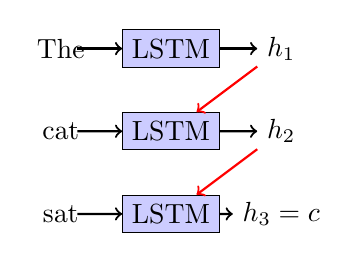
\begin{tikzpicture}[scale=0.7]
                % Words
                \node at (0, 0) {The};
                \node at (0, -1.5) {cat};
                \node at (0, -3) {sat};
                
                % LSTM cells
                \node[draw, rectangle, fill=blue!20] (lstm1) at (2, 0) {LSTM};
                \node[draw, rectangle, fill=blue!20] (lstm2) at (2, -1.5) {LSTM};
                \node[draw, rectangle, fill=blue!20] (lstm3) at (2, -3) {LSTM};
                
                % Hidden states
                \node (h1) at (4, 0) {$h_1$};
                \node (h2) at (4, -1.5) {$h_2$};
                \node (h3) at (4, -3) {$h_3 = c$};
                
                % Connections
                \draw[->, thick] (0.3, 0) -- (lstm1);
                \draw[->, thick] (0.3, -1.5) -- (lstm2);
                \draw[->, thick] (0.3, -3) -- (lstm3);
                
                \draw[->, thick] (lstm1) -- (h1);
                \draw[->, thick] (lstm2) -- (h2);
                \draw[->, thick] (lstm3) -- (h3);
                
                \draw[->, thick, red] (h1) -- (lstm2);
                \draw[->, thick, red] (h2) -- (lstm3);
            \end{tikzpicture}
        \end{column}
    \end{columns}
\end{frame}

\begin{frame}[t]{The Mathematics of Encoding}
    \motivation{
        Now let's formalize what we just saw intuitively
    }
    
    \textbf{Encoder equations (with explanations):}
    
    \eqbox{
        \textbf{For each input word $x_t$ at time $t$:}\\
        \vspace{0.3em}
        $h_t^{enc} = \text{LSTM}(x_t, h_{t-1}^{enc})$\\
        \vspace{0.3em}
        Where:
        \begin{itemize}
            \item $x_t$ = embedding of word at position $t$ (e.g., "cat" $\rightarrow$ [0.2, -0.1, ...])
            \item $h_{t-1}^{enc}$ = previous hidden state (what we understood so far)
            \item $h_t^{enc}$ = new hidden state (updated understanding)
        \end{itemize}
        \vspace{0.3em}
        \textbf{After processing all $T$ words:}\\
        \vspace{0.3em}
        $c = h_T^{enc}$ \quad (context vector = final understanding)
    }
    
    \vspace{0.5em}
    \textbf{Dimensions (crucial for implementation!):}
    \begin{itemize}
        \item Input embedding: $x_t \in \mathbb{R}^{d_{embed}}$ (typically 100-300)
        \item Hidden state: $h_t \in \mathbb{R}^{d_{hidden}}$ (typically 256-512)
        \item Context vector: $c \in \mathbb{R}^{d_{hidden}}$ (same as hidden!)
    \end{itemize}
\end{frame}

\begin{frame}[fragile,t]{Encoder Implementation (Simplified)}
    \motivation{
        Let's implement what we just learned - it's simpler than you think!
    }
    
    \begin{lstlisting}[language=Python]
class Encoder:
    def __init__(self, vocab_size, embed_dim, hidden_dim):
        # Initialize components
        self.embedding = Embedding(vocab_size, embed_dim)
        self.lstm = LSTM(embed_dim, hidden_dim)
        
    def forward(self, input_sequence):
        # input_sequence: list of word indices [5, 23, 67, ...]
        
        # Step 1: Convert words to embeddings
        embeddings = [self.embedding(word) for word in input_sequence]
        
        # Step 2: Process through LSTM
        hidden = zeros(hidden_dim)  # Initial state
        
        for embed in embeddings:
            hidden = self.lstm(embed, hidden)  # Update understanding
            
        # Step 3: Return final understanding
        context = hidden  # This is our context vector!
        return context
    \end{lstlisting}
    
    \checkpoint{
        What's the size of context if we have 10,000 input words? 10 words? 1 word?\\
        Answer: Always hidden\_dim! That's the beauty (and problem) of this approach.
    }
\end{frame}

\begin{frame}[t]{Building Intuition: The Decoder}
    \motivation{
        The decoder's job: Use the understanding to generate the translation
    }
    
    \textbf{Generation process (step-by-step):}
    
    \begin{columns}[T]
        \begin{column}{0.6\textwidth}
            \textbf{At each generation step:}
            \begin{enumerate}
                \item Start with context + previous word
                \item Compute new hidden state
                \item Predict next word probabilities
                \item Sample or take argmax
                \item Repeat until <END> token
            \end{enumerate}
            
            \vspace{0.5em}
            \textbf{Concrete example:} Generating "Le chat"
            \begin{itemize}
                \item Start: <START> + context $\rightarrow$ "Le"
                \item Step 1: "Le" + context $\rightarrow$ "chat"
                \item Step 2: "chat" + context $\rightarrow$ <END>
                \item Output: ["Le", "chat"]
            \end{itemize}
        \end{column}
        \begin{column}{0.4\textwidth}
            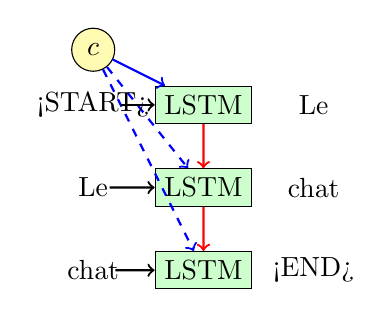
\begin{tikzpicture}[scale=0.7]
                % Context
                \node[draw, circle, fill=yellow!30] (context) at (0, 1) {$c$};
                
                % Decoder LSTMs
                \node[draw, rectangle, fill=green!20] (lstm1) at (2, 0) {LSTM};
                \node[draw, rectangle, fill=green!20] (lstm2) at (2, -1.5) {LSTM};
                \node[draw, rectangle, fill=green!20] (lstm3) at (2, -3) {LSTM};
                
                % Outputs
                \node at (4, 0) {Le};
                \node at (4, -1.5) {chat};
                \node at (4, -3) {<END>};
                
                % Context connections
                \draw[->, thick, blue] (context) -- (lstm1);
                \draw[->, thick, blue, dashed] (context) -- (lstm2);
                \draw[->, thick, blue, dashed] (context) -- (lstm3);
                
                % Sequential connections
                \draw[->, thick, red] (lstm1) -- (lstm2);
                \draw[->, thick, red] (lstm2) -- (lstm3);
                
                % Previous word connections
                \node at (0, 0) {<START>};
                \node at (0, -1.5) {Le};
                \node at (0, -3) {chat};
                
                \draw[->, thick] (0.5, 0) -- (lstm1);
                \draw[->, thick] (0.3, -1.5) -- (lstm2);
                \draw[->, thick] (0.4, -3) -- (lstm3);
            \end{tikzpicture}
        \end{column}
    \end{columns}
\end{frame}

\begin{frame}[t]{The Mathematics of Decoding}
    \motivation{
        Let's formalize the generation process
    }
    
    \textbf{Decoder equations (with explanations):}
    
    \eqbox{
        \textbf{For each output position $t$:}\\
        \vspace{0.3em}
        $h_t^{dec} = \text{LSTM}(y_{t-1}, h_{t-1}^{dec}, c)$\\
        \vspace{0.3em}
        Where:
        \begin{itemize}
            \item $y_{t-1}$ = previous generated word (or <START> if $t=1$)
            \item $h_{t-1}^{dec}$ = previous decoder hidden state
            \item $c$ = context vector from encoder (always the same!)
        \end{itemize}
        \vspace{0.3em}
        \textbf{To predict next word:}\\
        \vspace{0.3em}
        $P(y_t | y_{<t}, c) = \softmax(W \cdot h_t^{dec} + b)$\\
        \vspace{0.3em}
        This gives probability for each word in vocabulary!
    }
    
    \misconception{
        \textbf{Common mistake:} "The decoder only uses context once"\\
        \textbf{Truth:} Context $c$ is fed at EVERY step of generation!
    }
\end{frame}

\begin{frame}[fragile,t]{Decoder Implementation (Simplified)}
    \begin{lstlisting}[language=Python]
class Decoder:
    def __init__(self, vocab_size, embed_dim, hidden_dim):
        self.embedding = Embedding(vocab_size, embed_dim)
        self.lstm = LSTM(embed_dim + hidden_dim, hidden_dim)  # Note: larger input!
        self.output_projection = Linear(hidden_dim, vocab_size)
        
    def forward(self, context, max_length=50):
        outputs = []
        hidden = context  # Initialize with context
        word = START_TOKEN
        
        for _ in range(max_length):
            # Step 1: Embed previous word
            embed = self.embedding(word)
            
            # Step 2: Combine with context and process
            lstm_input = concatenate([embed, context])  # Key: use context always!
            hidden = self.lstm(lstm_input, hidden)
            
            # Step 3: Predict next word
            logits = self.output_projection(hidden)
            probs = softmax(logits)
            word = argmax(probs)  # Or sample from probs
            
            outputs.append(word)
            if word == END_TOKEN:
                break
                
        return outputs
    \end{lstlisting}
\end{frame}

\begin{frame}[t]{Training: Teacher Forcing}
    \motivation{
        How do we train this model? We can't wait for it to generate everything!
    }
    
    \textbf{The Teacher Forcing trick:}
    
    \begin{columns}[T]
        \begin{column}{0.5\textwidth}
            \textbf{During Training:}
            \begin{itemize}
                \item Feed the TRUE previous word
                \item Not the model's prediction
                \item This speeds up training dramatically
                \item Prevents error accumulation
            \end{itemize}
            
            \vspace{0.5em}
            Example: Teaching "Le chat noir"
            \begin{itemize}
                \item Step 1: <START> $\rightarrow$ predict "Le"
                \item Step 2: "Le" (true) $\rightarrow$ predict "chat"
                \item Step 3: "chat" (true) $\rightarrow$ predict "noir"
            \end{itemize}
        \end{column}
        \begin{column}{0.5\textwidth}
            \textbf{During Inference:}
            \begin{itemize}
                \item Feed the MODEL's previous prediction
                \item No true words available!
                \item Errors can accumulate
                \item Need beam search to help
            \end{itemize}
            
            \vspace{0.5em}
            Example: Generating translation
            \begin{itemize}
                \item Step 1: <START> $\rightarrow$ generates "Le"
                \item Step 2: "Le" (generated) $\rightarrow$ generates "chat"
                \item Step 3: "chat" (generated) $\rightarrow$ generates "noir"
            \end{itemize}
        \end{column}
    \end{columns}
    
    \checkpoint{
        Why might teacher forcing cause problems during deployment?\\
        Hint: The model never learns to recover from its own mistakes!
    }
\end{frame}

%=====================================
% PART 3: THE INFORMATION BOTTLENECK PROBLEM
%=====================================

\section{Part 3: The Information Bottleneck Problem}

\begin{frame}[t]{When Seq2Seq Fails}
    \motivation{
        Seq2Seq works great for short sentences. But what about long ones?
    }
    
    \textbf{The Compression Problem:}
    
    \begin{center}
    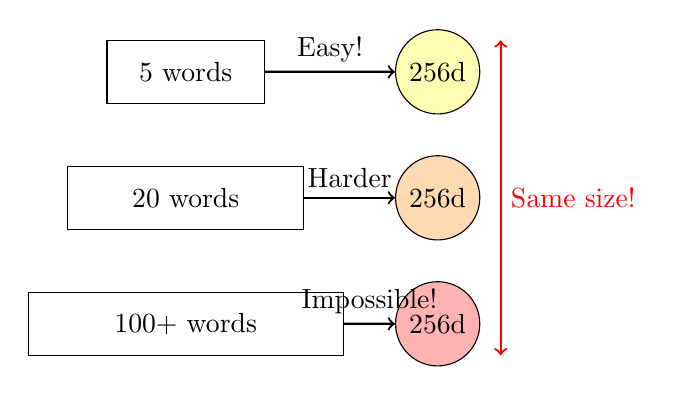
\begin{tikzpicture}[scale=0.8]
        % Short sentence
        \node[draw, rectangle, minimum width=2cm, minimum height=0.8cm] (short) at (0, 2) {5 words};
        \node[draw, circle, fill=yellow!30] (context1) at (4, 2) {256d};
        \draw[->, thick] (short) -- (context1) node[midway, above] {Easy!};
        
        % Medium sentence
        \node[draw, rectangle, minimum width=3cm, minimum height=0.8cm] (medium) at (0, 0) {20 words};
        \node[draw, circle, fill=orange!30] (context2) at (4, 0) {256d};
        \draw[->, thick] (medium) -- (context2) node[midway, above] {Harder};
        
        % Long sentence
        \node[draw, rectangle, minimum width=4cm, minimum height=0.8cm] (long) at (0, -2) {100+ words};
        \node[draw, circle, fill=red!30] (context3) at (4, -2) {256d};
        \draw[->, thick] (long) -- (context3) node[midway, above] {Impossible!};
        
        % Same size indicator
        \draw[<->, thick, red] (5, 2.5) -- (5, -2.5) node[midway, right] {Same size!};
    \end{tikzpicture}
    \end{center}
    
    \textbf{Information Theory Perspective:}
    \begin{itemize}
        \item Each word: $\approx$ 10 bits of information
        \item 100 words: 1000 bits of information
        \item 256-dim vector: $\approx$ 256 bits capacity
        \item \highlight{We're losing 75\% of the information!}
    \end{itemize}
\end{frame}

\begin{frame}[t]{Visualizing Information Loss}
    \textbf{What gets lost in long sequences?}
    
    \begin{columns}[T]
        \begin{column}{0.5\textwidth}
            \textbf{Original paragraph:}
            \small
            "The International Conference on Machine Learning, which is one of the premier venues for presenting research in machine learning and attracts submissions from researchers around the world working on various aspects of learning algorithms, accepted our paper about using neural networks for natural language understanding."
        \end{column}
        \begin{column}{0.5\textwidth}
            \textbf{What the context captures:}
            \begin{itemize}
                \item \checkmark General topic (ML conference)
                \item \checkmark Sentiment (positive - accepted)
                \item \texttimes Specific conference name
                \item \texttimes "researchers around the world"
                \item \texttimes "neural networks" detail
                \item \texttimes Word order/grammar structure
            \end{itemize}
            
            \vspace{0.5em}
            \misconception{
                \textbf{Wrong:} "Just use a bigger context vector!"\\
                \textbf{Problem:} Even 1024d isn't enough for books!
            }
        \end{column}
    \end{columns}
    
    \vspace{0.5em}
    \textbf{Experimental Evidence (Bahdanau et al., 2015):}
    \begin{center}
    \begin{tabular}{|l|c|c|c|}
        \hline
        \textbf{Sentence Length} & \textbf{BLEU Score} & \textbf{Quality} \\
        \hline
        < 10 words & 35.2 & Excellent \\
        10-20 words & 28.5 & Good \\
        20-30 words & 19.3 & Mediocre \\
        > 30 words & 9.7 & Poor \\
        \hline
    \end{tabular}
    \end{center}
\end{frame}

\begin{frame}[t]{The Bottleneck Visualization}
    \begin{center}
    %\includegraphics[width=0.8\textwidth]{../figures/bottleneck_visualization.pdf}
    
    \vspace{0.5em}
    \textit{[Bottleneck visualization showing information flow]}
    \end{center}
    
    \textbf{Key Insights:}
    \begin{enumerate}
        \item Early words get "overwritten" by later ones
        \item Middle information gets averaged out
        \item Final words dominate the context vector
        \item Decoder forgets the beginning by the end!
    \end{enumerate}
    
    \checkpoint{
        If you were designing a solution, what would you do?\\
        Think: How do humans handle long texts when translating?
    }
\end{frame}

%=====================================
% PART 4: ATTENTION MECHANISM - THE GAME CHANGER
%=====================================

\section{Part 4: Attention Mechanism - The Game Changer}

\begin{frame}[t]{The Key Insight: Look Back!}
    \motivation{
        What if the decoder could look back at ALL encoder states, not just the final one?
    }
    
    \textbf{Human Translation Process:}
    
    When translating "The black cat sat on the mat" $\rightarrow$ "Le chat noir..."
    
    \begin{center}
    \begin{tabular}{|l|l|}
        \hline
        \textbf{Generating} & \textbf{Looking at} \\
        \hline
        "Le" & Mainly "The" \\
        "chat" & Mainly "cat" \\
        "noir" & Mainly "black" \\
        "s'est assis" & Mainly "sat" \\
        "sur" & Mainly "on" \\
        "le" & Mainly "the" \\
        "tapis" & Mainly "mat" \\
        \hline
    \end{tabular}
    \end{center}
    
    \textbf{The Attention Solution:}
    \begin{itemize}
        \item Keep ALL encoder hidden states $h_1^{enc}, h_2^{enc}, ..., h_T^{enc}$
        \item At each decoder step, decide which ones are relevant
        \item Create a weighted combination based on relevance
        \item Use this custom context for each word!
    \end{itemize}
\end{frame}

\begin{frame}[t]{How Attention Works (Intuition)}
    \textbf{The 3-step attention process:}
    
    \begin{enumerate}
        \item \textbf{Score:} How relevant is each encoder state?
        \begin{itemize}
            \item Current decoder state: $h_t^{dec}$ (what we're generating)
            \item Each encoder state: $h_i^{enc}$ (source word $i$)
            \item Score: $e_{ti} = \text{score}(h_t^{dec}, h_i^{enc})$
        \end{itemize}
        
        \item \textbf{Normalize:} Convert scores to probabilities
        \begin{itemize}
            \item Apply softmax: $\alpha_{ti} = \frac{\exp(e_{ti})}{\sum_j \exp(e_{tj})}$
            \item Now $\sum_i \alpha_{ti} = 1$ (probability distribution!)
        \end{itemize}
        
        \item \textbf{Combine:} Weighted sum of encoder states
        \begin{itemize}
            \item Context: $c_t = \sum_i \alpha_{ti} \cdot h_i^{enc}$
            \item Different context for each decoder step $t$!
        \end{itemize}
    \end{enumerate}
    
    \checkpoint{
        Why do we use softmax instead of just normalizing by sum?\\
        Hint: Softmax makes differences more pronounced!
    }
\end{frame}

\begin{frame}[t]{Attention Mathematics (Step by Step)}
    \motivation{
        Let's see the exact equations with concrete numbers
    }
    
    \textbf{Example: Generating "chat" when translating "The cat sat"}
    
    \eqbox{
        \textbf{Step 1: Score each source word}\\
        Current decoder state: $h_2^{dec}$ = [0.5, -0.2, 0.8]\\
        \vspace{0.3em}
        \begin{tabular}{lll}
            $e_{2,1} = h_2^{dec} \cdot h_1^{enc}$ & = [0.5,-0.2,0.8] $\cdot$ [0.1,0.2,0.1] & = 0.09 \\
            $e_{2,2} = h_2^{dec} \cdot h_2^{enc}$ & = [0.5,-0.2,0.8] $\cdot$ [0.8,0.1,0.7] & = 0.94 \\
            $e_{2,3} = h_2^{dec} \cdot h_3^{enc}$ & = [0.5,-0.2,0.8] $\cdot$ [0.2,0.3,0.2] & = 0.20 \\
        \end{tabular}
    }
    
    \eqbox{
        \textbf{Step 2: Convert to probabilities}\\
        $\alpha_{2,1} = \frac{e^{0.09}}{e^{0.09} + e^{0.94} + e^{0.20}} = \frac{1.09}{4.04} = 0.27$\\
        $\alpha_{2,2} = \frac{e^{0.94}}{4.04} = 0.63$ \quad \highlight{Highest attention on "cat"!}\\
        $\alpha_{2,3} = \frac{e^{0.20}}{4.04} = 0.10$
    }
    
    \eqbox{
        \textbf{Step 3: Compute context}\\
        $c_2 = 0.27 \cdot h_1^{enc} + 0.63 \cdot h_2^{enc} + 0.10 \cdot h_3^{enc}$
    }
\end{frame}

\begin{frame}[t]{Different Attention Mechanisms}
    \textbf{Three main ways to compute attention scores:}
    
    \begin{enumerate}
        \item \textbf{Dot Product (Luong):}
        \eqbox{
            $e_{ti} = h_t^{dec} \cdot h_i^{enc}$\\
            Fast, simple, works well
        }
        
        \item \textbf{Scaled Dot Product (Transformer):}
        \eqbox{
            $e_{ti} = \frac{h_t^{dec} \cdot h_i^{enc}}{\sqrt{d}}$\\
            Prevents values from getting too large
        }
        
        \item \textbf{Additive/Concat (Bahdanau):}
        \eqbox{
            $e_{ti} = v^T \cdot \tanh(W_1 h_t^{dec} + W_2 h_i^{enc})$\\
            More parameters, more flexible
        }
    \end{enumerate}
    
    \misconception{
        \textbf{Common confusion:} "Attention looks at future words"\\
        \textbf{Truth:} Decoder attention only looks at encoder states (source), never at future target words!
    }
\end{frame}

\begin{frame}[fragile,t]{Attention Implementation}
    \begin{lstlisting}[language=Python]
def attention(decoder_hidden, encoder_outputs):
    """
    decoder_hidden: current decoder state [hidden_dim]
    encoder_outputs: all encoder states [seq_len, hidden_dim]
    """
    # Step 1: Compute scores
    scores = []
    for enc_output in encoder_outputs:
        score = dot_product(decoder_hidden, enc_output)
        scores.append(score)
    
    # Step 2: Normalize with softmax
    scores = np.array(scores)
    exp_scores = np.exp(scores - np.max(scores))  # Stability trick
    attention_weights = exp_scores / np.sum(exp_scores)
    
    # Step 3: Compute weighted sum
    context = np.zeros_like(decoder_hidden)
    for weight, enc_output in zip(attention_weights, encoder_outputs):
        context += weight * enc_output
    
    return context, attention_weights

# Usage in decoder:
context, weights = attention(current_hidden, all_encoder_states)
# Now use context instead of fixed context vector!
    \end{lstlisting}
\end{frame}

\begin{frame}[t]{Visualizing Attention}
    \begin{center}
    %\includegraphics[width=0.7\textwidth]{../figures/attention_heatmap.pdf}
    
    \textit{[Attention heatmap visualization]}
    \end{center}
    
    \textbf{What the visualization tells us:}
    \begin{itemize}
        \item Diagonal pattern = word-to-word alignment
        \item Off-diagonal = reordering (common in translation)
        \item Distributed attention = phrase translation
        \item Sharp attention = direct word correspondence
    \end{itemize}
    
    \checkpoint{
        Look at "s'est assis" attending to "sat" - why two words for one?
    }
\end{frame}

\begin{frame}[t]{The Impact of Attention}
    \textbf{Performance Improvements (Bahdanau et al., 2015):}
    
    \begin{center}
    \begin{tabular}{|l|c|c|c|}
        \hline
        \textbf{Model} & \textbf{Short (<10)} & \textbf{Medium (10-20)} & \textbf{Long (>20)} \\
        \hline
        Seq2Seq & 35.2 & 28.5 & 9.7 \\
        Seq2Seq + Attention & 36.1 & 34.8 & 28.3 \\
        \hline
        Improvement & +2.6\% & +22.1\% & \highlight{+192\%} \\
        \hline
    \end{tabular}
    \end{center}
    
    \vspace{0.5em}
    \textbf{Why attention helps so much:}
    \begin{enumerate}
        \item No information bottleneck - access all source information
        \item Handles long sequences - doesn't forget the beginning
        \item Provides interpretability - see what model focuses on
        \item Enables better gradient flow - shorter paths
    \end{enumerate}
    
    \motivation{
        This single innovation led directly to Transformers ("Attention is All You Need") and ultimately to GPT, BERT, and modern LLMs!
    }
\end{frame}

%=====================================
% APPENDIX A: MATHEMATICAL DEEP DIVE
%=====================================

\section{Appendix A: Mathematical Deep Dive}

\begin{frame}[t]{Complete Seq2Seq Mathematics}
    \textbf{Full mathematical formulation:}
    
    \small
    \textbf{Encoder:}
    \begin{align}
        h_t^{enc} &= \text{LSTM}^{enc}(E^{enc}(x_t), h_{t-1}^{enc}) \\
        c &= h_T^{enc}
    \end{align}
    
    \textbf{Decoder without Attention:}
    \begin{align}
        h_t^{dec} &= \text{LSTM}^{dec}([E^{dec}(y_{t-1}); c], h_{t-1}^{dec}) \\
        P(y_t | y_{<t}, X) &= \softmax(W_o h_t^{dec} + b_o)
    \end{align}
    
    \textbf{Decoder with Attention:}
    \begin{align}
        e_{ti} &= \text{score}(h_t^{dec}, h_i^{enc}) \\
        \alpha_{ti} &= \frac{\exp(e_{ti})}{\sum_{j=1}^T \exp(e_{tj})} \\
        c_t &= \sum_{i=1}^T \alpha_{ti} h_i^{enc} \\
        h_t^{dec} &= \text{LSTM}^{dec}([E^{dec}(y_{t-1}); c_t], h_{t-1}^{dec}) \\
        P(y_t | y_{<t}, X) &= \softmax(W_o [h_t^{dec}; c_t] + b_o)
    \end{align}
\end{frame}

\begin{frame}[t]{Training Objectives}
    \textbf{Loss Function:}
    
    \eqbox{
        \textbf{Cross-entropy loss over entire sequence:}\\
        \vspace{0.3em}
        $\mathcal{L} = -\sum_{t=1}^{T'} \log P(y_t^* | y_{<t}^*, X)$\\
        \vspace{0.3em}
        Where $y^*$ is the true target sequence
    }
    
    \textbf{Training Process:}
    \begin{enumerate}
        \item Forward pass: Encode source, decode with teacher forcing
        \item Compute loss at each time step
        \item Backpropagate through entire network
        \item Update parameters with optimizer (Adam, SGD)
    \end{enumerate}
    
    \textbf{Key Hyperparameters:}
    \begin{itemize}
        \item Hidden dimension: 256-512 (trade-off: capacity vs speed)
        \item Embedding dimension: 100-300 (semantic richness)
        \item Vocabulary size: 10K-50K (coverage vs efficiency)
        \item Dropout rate: 0.2-0.3 (prevent overfitting)
        \item Learning rate: 0.001 (with decay)
    \end{itemize}
\end{frame}

\begin{frame}[fragile,t]{Beam Search Algorithm}
    \motivation{
        Greedy decoding often produces suboptimal translations. Beam search explores multiple paths!
    }
    
    \textbf{Algorithm (Pseudocode):}
    \small
    \begin{lstlisting}[language=Python, basicstyle=\ttfamily\tiny]
# Input: Encoder outputs, beam size k
beams = [(<START>, 0.0)]

while not all_beams_ended:
    new_beams = []
    for (sequence, score) in beams:
        if last_token(sequence) == <END>:
            add_to_completed(sequence, score)
        else:
            probs = decode_step(sequence)
            top_k = get_top_k_tokens(probs, k)
            for token, prob in top_k:
                new_seq = sequence + [token]
                new_score = score + log(prob)
                new_beams.append((new_seq, new_score))
    
    beams = select_top_k_beams(new_beams, k)

return best_completed_sequence()
    \end{lstlisting}
\end{frame}

\begin{frame}[t]{BLEU Score Computation}
    \textbf{Evaluating Translation Quality:}
    
    \eqbox{
        \textbf{BLEU = Bilingual Evaluation Understudy}\\
        \vspace{0.3em}
        BLEU = BP $\cdot$ exp$\left(\sum_{n=1}^4 w_n \log p_n\right)$\\
        \vspace{0.3em}
        Where:
        \begin{itemize}
            \item $p_n$ = precision of n-grams
            \item $w_n$ = weights (usually 0.25 each)
            \item BP = brevity penalty (penalizes short translations)
        \end{itemize}
    }
    
    \textbf{Example:}
    \begin{itemize}
        \item Reference: "The cat sat on the mat"
        \item Hypothesis: "The cat is on the mat"
        \item 1-gram precision: 5/6 = 0.83 (words)
        \item 2-gram precision: 2/5 = 0.40 (bigrams)
        \item BLEU-2 $\approx$ 0.57
    \end{itemize}
    
    \checkpoint{
        Why do we use geometric mean (exp of log sum) instead of arithmetic mean?
    }
\end{frame}

%=====================================
% APPENDIX B: MODERN APPLICATIONS (2024)
%=====================================

\section{Appendix B: Modern Applications (2024)}

\begin{frame}[t]{Seq2Seq in 2024: Where It's Used}
    \begin{center}
    %\includegraphics[width=0.9\textwidth]{../figures/applications_2024.pdf}
    
    \textit{[Modern applications grid visualization]}
    \end{center}
    
    \textbf{Current Applications:}
    \begin{columns}[T]
        \begin{column}{0.5\textwidth}
            \textbf{Text-to-Text:}
            \begin{itemize}
                \item Machine Translation (Google Translate)
                \item Text Summarization
                \item Question Answering
                \item Dialogue Systems
            \end{itemize}
            
            \textbf{Speech:}
            \begin{itemize}
                \item Speech Recognition (Whisper)
                \item Speech Synthesis
                \item Voice Translation
            \end{itemize}
        \end{column}
        \begin{column}{0.5\textwidth}
            \textbf{Code:}
            \begin{itemize}
                \item Code Generation (GitHub Copilot)
                \item Code Translation
                \item Bug Fixing
                \item Documentation Generation
            \end{itemize}
            
            \textbf{Multimodal:}
            \begin{itemize}
                \item Image Captioning
                \item Video Description
                \item Visual Question Answering
            \end{itemize}
        \end{column}
    \end{columns}
\end{frame}

\begin{frame}[t]{From Seq2Seq to Transformers}
    \textbf{The Evolution Path:}
    
    \begin{center}
    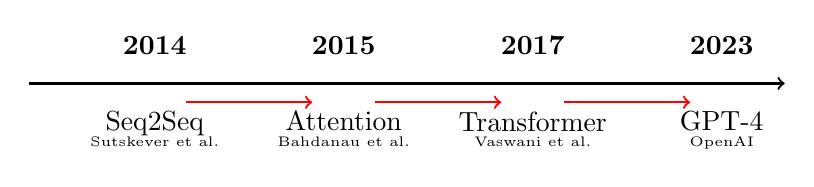
\begin{tikzpicture}[scale=0.8]
        % Timeline
        \draw[thick, ->] (0,0) -- (12,0);
        
        % Milestones
        \node[above] at (2,0.3) {\textbf{2014}};
        \node[below] at (2,-0.3) {Seq2Seq};
        \node[below] at (2,-0.7) {\tiny Sutskever et al.};
        
        \node[above] at (5,0.3) {\textbf{2015}};
        \node[below] at (5,-0.3) {Attention};
        \node[below] at (5,-0.7) {\tiny Bahdanau et al.};
        
        \node[above] at (8,0.3) {\textbf{2017}};
        \node[below] at (8,-0.3) {Transformer};
        \node[below] at (8,-0.7) {\tiny Vaswani et al.};
        
        \node[above] at (11,0.3) {\textbf{2023}};
        \node[below] at (11,-0.3) {GPT-4};
        \node[below] at (11,-0.7) {\tiny OpenAI};
        
        % Connections
        \draw[->, thick, red] (2.5,-0.3) -- (4.5,-0.3);
        \draw[->, thick, red] (5.5,-0.3) -- (7.5,-0.3);
        \draw[->, thick, red] (8.5,-0.3) -- (10.5,-0.3);
    \end{tikzpicture}
    \end{center}
    
    \textbf{Key Innovations:}
    \begin{itemize}
        \item Seq2Seq: Separate encoding and decoding
        \item +Attention: Solve the bottleneck problem
        \item Transformer: Attention is ALL you need (no RNNs!)
        \item GPT/BERT: Pre-training on massive data
    \end{itemize}
    
    \motivation{
        The seq2seq architecture you learned today is the foundation of ALL modern LLMs!
    }
\end{frame}

\begin{frame}[t]{Limitations and Future Directions}
    \textbf{Current Limitations of Seq2Seq:}
    \begin{enumerate}
        \item \textbf{Sequential processing:} Can't parallelize
        \item \textbf{Fixed vocabulary:} Can't handle new words
        \item \textbf{No pre-training:} Trains from scratch
        \item \textbf{Single modality:} Text only (originally)
    \end{enumerate}
    
    \vspace{0.5em}
    \textbf{How Modern Models Address These:}
    \begin{itemize}
        \item Transformers: Full parallelization
        \item Subword tokenization: Handle any word
        \item Pre-training: Transfer learning
        \item Multimodal: Vision + Language models
    \end{itemize}
    
    \checkpoint{
        Based on what you learned, what would YOU improve about seq2seq?
    }
\end{frame}

% Summary slide
\begin{frame}[t]{Week 4 Summary: Key Takeaways}
    \begin{columns}[T]
        \begin{column}{0.5\textwidth}
            \textbf{What We Learned:}
            \begin{enumerate}
                \item Variable-length problem
                \item Encoder-Decoder solution
                \item Information bottleneck
                \item Attention mechanism
                \item Implementation details
            \end{enumerate}
            
            \vspace{0.5em}
            \textbf{Key Equations:}
            \begin{itemize}
                \item Encoding: $h_t = \text{LSTM}(x_t, h_{t-1})$
                \item Attention: $\alpha_t = \softmax(e_t)$
                \item Context: $c_t = \sum \alpha_{ti} h_i$
            \end{itemize}
        \end{column}
        \begin{column}{0.5\textwidth}
            \textbf{Practical Skills:}
            \begin{itemize}
                \item Implement encoder-decoder
                \item Add attention mechanism
                \item Use teacher forcing
                \item Apply beam search
                \item Evaluate with BLEU
            \end{itemize}
            
            \vspace{0.5em}
            \textbf{Next Week:}
            \begin{itemize}
                \item Transformers!
                \item Self-attention
                \item Multi-head attention
                \item Positional encoding
                \item "Attention is All You Need"
            \end{itemize}
        \end{column}
    \end{columns}
    
    \vspace{0.5em}
    \motivation{
        You now understand the foundation of modern NLP! Everything from Google Translate to ChatGPT builds on these concepts.
    }
\end{frame}

\end{document}